
\title{T-61.5130 Machine Learning and Neural Networks}
\author{Karhunen, Luttinen}
\date{Exercise 7}

\newcommand{\vect}[1]{{\bf{#1}}}
\newcommand{\svect}[1]{\boldsymbol{#1}}
\newcommand{\matr}[1]{\boldsymbol{#1}}

\usepackage{graphicx}

\begin{document}

\maketitle
\thispagestyle{empty}

\begin{enumerate}

\item Consider on a general level the major differences (and similarities)
  between radial-basis function (RBF) networks and multilayer perceptron
  (MLP) networks.

  \begin{solution}

    \begin{itemize}
    \item Both RBF and MLP networks are nonlinear layered networks having
      universal approximation properties (that is, they are able to
      approximate any smooth enough function to an arbitrary degree of accuracy).
    \item The most important differences between them are:
      % 
      \begin{enumerate}
      \item An RBF network has a single hidden layer, while an MLP can have
        several hidden layers.
      \item The computational nodes in the MLP network are similar in various layers,
        while in the RBF network they are quite different in the output
        and hidden layers.
      \item In the RBF network, the output layer is linear, while it is usually
        nonlinear in an MLP network.
      \item In each hidden node, the activation function of RBF network computes
        an {\em Euclidean distance}, while in MLP networks an {\em inner product}
        between the input and the weight vector is computed.
      \item MLPs construct {\em global} approximations, while RBF networks
        approximate {\em locally} nonlinear input-output mappings.
        % Jaakko: The basis functions can be global, aren't the
        % approximations of RBFnets then global???
      \end{enumerate}
      % 
    \item MLP may require less parameters than the RBF network for achieving
      the same accuracy.
      % Jaakko: Citation needed!! Or a reason / proof / argumentation.
    \end{itemize}

  \end{solution}

\item Derive the equation for learning the weights of RBF networks
  with several neurons in the output layer.

  % In Ham's and Kostanic's book, training of RBF networks is
  % considered for the
  % case of a single neuron in the output layer only. Show how the
  % learning method
  % presented in section 3.6.1 can be generalized for several neurons
  % in the
  % output layer.

  \begin{solution}

    The $n$-th output of an RBF network for input $\mathbf{x}$ is
    \begin{align*}
      y_n(\mathbf{x}) = \sum^D_{d=1} w_{dn}
      \phi_d(\|\mathbf{x}-\mathbf{c}_d\|), \quad n=1,\ldots,N,
    \end{align*}
    where $\mathbf{c}_d$ are the cluster centers, $\phi_d$ the radial
    basis functions and $w_{dn}$ the weights.  Let us assume that we
    have a set of $M$ input-output pairs $(\hat{\mathbf{x}}_k,
    \hat{\mathbf{y}}_k)$.  Then our set of equations becomes
    \begin{align*}
      \underbrace{
        \begin{bmatrix}
          \hat{y}_{11} & \ldots & \hat{y}_{1N}
          \\
          \vdots & \ddots & \vdots
          \\
          \hat{y}_{M1} & \ldots & \hat{y}_{MN}
        \end{bmatrix}
      }_{\mathbf{Y}}
      &=
      \underbrace{
        \begin{bmatrix}
          \phi_1(\|\hat{\mathbf{x}}_1-\mathbf{c}_1\|) & \ldots &
          \phi_D(\|\hat{\mathbf{x}}_1-\mathbf{c}_D\|) 
          \\
          \vdots & \ddots & \vdots
          \\
          \phi_1(\|\hat{\mathbf{x}}_M-\mathbf{c}_1\|) & \ldots &
          \phi_D(\|\hat{\mathbf{x}}_M-\mathbf{c}_D\|)
        \end{bmatrix}
      }_{\mathbf{\Phi}}
      \underbrace{
        \begin{bmatrix}
          w_{11} & \ldots & w_{1N}
          \\
          \vdots & \ddots & \vdots
          \\
          w_{D1} & \ldots & w_{DN}
        \end{bmatrix}
      }_{\mathbf{W}}
    \end{align*}
    Note that $\mathbf{Y}$, $\mathbf{W}$ and $\mathbf{\Phi}$ are $M
    \times N$, $M \times D$ and $D \times N$ matrices, respectively.
    $M$ is the number of data points, $N$ is the dimensionality of the
    output vectors and $D$ is the number of neurons in the hidden
    layer.  The optimal solution can be found using the
    pseudo-inverse:
    \begin{align*}
      \mathbf{W} = (\mathbf{\Phi}^T\mathbf{\Phi})^{-1} \mathbf{\Phi}^T
      \mathbf{Y} = \mathbf{\Phi}^{\dagger} \mathbf{Y}.
    \end{align*}
    Note that this learns the weights only in the output layer.  If
    there are parameters in the radial basis functions, they need to
    be learnt using optimization methods.

  \end{solution}


\item The well-known XOR (Exclusive OR) problem is the simplest example of a
  two-class classification problem where the pattern vectors are not linearly
  separable. In the XOR problem, there are four two-dimensional input vectors
  (patterns) (-1,-1), (-1,1), (1,1), and (1,-1). The first and third pattern
  vector belong to the class 1, while the second and the fourth one belong
  to the class 2. Solve the XOR problem by using a RBF network with two
  Gaussian basis functions centered at ${\bf t}_1 = (-1,1)^T$ and
  ${\bf t}_2 = (1,-1)^T$.

  \begin{solution}

    RBF network for solving the XOR problem

    \begin{center}
      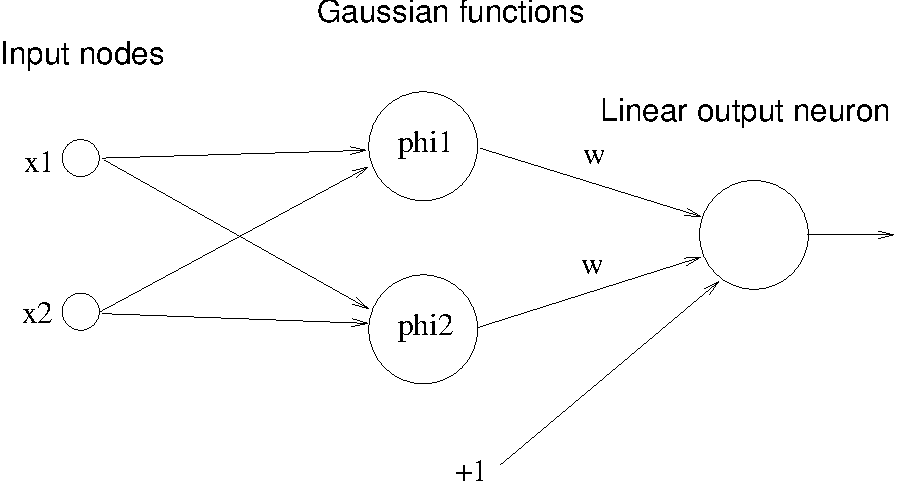
\includegraphics[scale=0.7]{v102-f1}
    \end{center}

    % Some notes on the above network:
    % \begin{itemize}
    % \item weight sharing is justified by the symmetry of the problem
    % \item the desired output values of the problem have nonzero mean and
    %   thus the output unit includes a bias 
    % \end{itemize}

    % Let us assume that the logical symbol 0 is represented by level -1
    % and symbol 1 is represented by level +1. Sometimes this is directly
    % taken as the XOR problem.

    \begin{enumerate}
    \item For the input pattern $\mathbf{x}=(-1,-1)^T$:
      \begin{eqnarray*}
        (1)\;G(\|\mathbf{x}-\mathbf{t}_1\|)&=&e^{-\|(-1,-1)^T-(-1,1)^T\|^2}\\
        &=&e^{-\|(0,-2)^T\|^2}=e^{-4}=0.01832\\
        (2)\;G(\|\mathbf{x}-\mathbf{t}_2\|)&=&e^{-\|(-1,-1)^T-(1,-1)^T\|^2}\\
        &=&e^{-\|(-2,0)^T\|^2}=e^{-4}=0.01832
      \end{eqnarray*}

    \item For the input pattern $\mathbf{x}=(-1,1)^T$:
      \begin{eqnarray*}
        (3)\;G(\|\mathbf{x}-\mathbf{t}_1\|)&=&e^{-\|(-1,1)^T-(-1,1)^T\|^2}\\
        &=&e^{-\|(0,0)^T\|^2}=e^{-0}=1\\
        (4)\;G(\|\mathbf{x}-\mathbf{t}_2\|)&=&e^{-\|(-1,1)^T-(1,-1)^T\|^2}\\
        &=&e^{-\|(-2,2)^T\|^2}=e^{-8}=0.000336
      \end{eqnarray*}

    \item For the input pattern $\mathbf{x}=(1,1)^T$:
      \begin{eqnarray*}
        (5)\;G(\|\mathbf{x}-\mathbf{t}_1\|)&=&e^{-\|(1,1)^T-(-1,1)^T\|^2}\\
        &=&e^{-\|(2,0)^T\|^2}=e^{-4}=0.01832\\
        (6)\;G(\|\mathbf{x}-\mathbf{t}_2\|)&=&e^{-\|(1,1)^T-(1,-1)^T\|^2}\\
        &=&e^{-\|(0,2)^T\|^2}=e^{-4}=0.01832
      \end{eqnarray*}

    \item For the input pattern $\mathbf{x}=(1,-1)^T$:
      \begin{eqnarray*}
        (7)\;G(\|\mathbf{x}-\mathbf{t}_1\|)&=&e^{-\|(1,-1)^T-(-1,1)^T\|^2}\\
        &=&e^{-\|(2,-2)^T\|^2}=e^{-8}=0.000336\\
        (8)\;G(\|\mathbf{x}-\mathbf{t}_2\|)&=&e^{-\|(1,-1)^T-(1,-1)^T\|^2}\\
        &=&e^{-\|(-0,0)^T\|^2}=e^{-0}=1
      \end{eqnarray*}
    \end{enumerate}

    Results (1)-(8) are combinded as a matrix
    \begin{equation*}
      \mathbf{G}=\begin{array}{cl}
        \begin{array}{ccc}
          \varphi_1(\mathbf{x})&\varphi_2(\mathbf{x})&\mbox{bias}
        \end{array} &\\
        \left[
          \begin{array}{ccc}
            e^{-4} & e^{-4} & 1\\
            1 & e^{-8}& 1\\
            e^{-4} & e^{-4} & 1\\
            e^{-8}& 1 & 1
          \end{array}
        \right] &
        \begin{array}{r}
          \mbox{ pattern }(-1,-1)\\
          (-1,1)\\
          (1,1)\\
          (1,-1)
        \end{array}
      \end{array}
    \end{equation*}
    and the desired responses as vector $d=(-1,1,-1,1)^T$, where we
    have chosen $-1$ and $1$ to represent classes 1 and 2,
    respectively.

    The linear parameters of the network are defined by
    \begin{equation*}
      \mathbf{Gw}=\mathbf{d}\mbox{, where }\mathbf{w}=(w,\;w,\;b)^T.
    \end{equation*}

    The solution to the equation is
    $\mathbf{w}=\mathbf{G}^\dagger\mathbf{d}$, where
    $\mathbf{G}^\dagger=(\mathbf{G}^T\mathbf{G})^{-1}\mathbf{G}^T$ is
    the pseudo inverse of $\mathbf{G}$

    \begin{equation*}
      \mathbf{G}^\dagger=
      \left[
        \begin{array}{rrrr}
          -0.5188 & 1.0190 & -0.5188 &0.0187\\
          -0.5188 & 0.0187 & -0.5188 &1.0190\\
          -0.5190 & -0.0190 & -0.5190 &-0.0190
        \end{array}\right]
    \end{equation*}
    \begin{equation*}
      \mathbf{w}=(2.0753,\;2.0753,\;-1.076)^T
    \end{equation*}


  \end{solution}


\item (demo) Compare the performance of LMS, MLP and RBF networks for
  the double-moon classification problem.

  \begin{solution}
    The following figures are from Simon Haykin \emph{Neural Networks
      and Learning Machines (Third Edition)} 2009 (Pearson Education).
    
    \begin{center}
      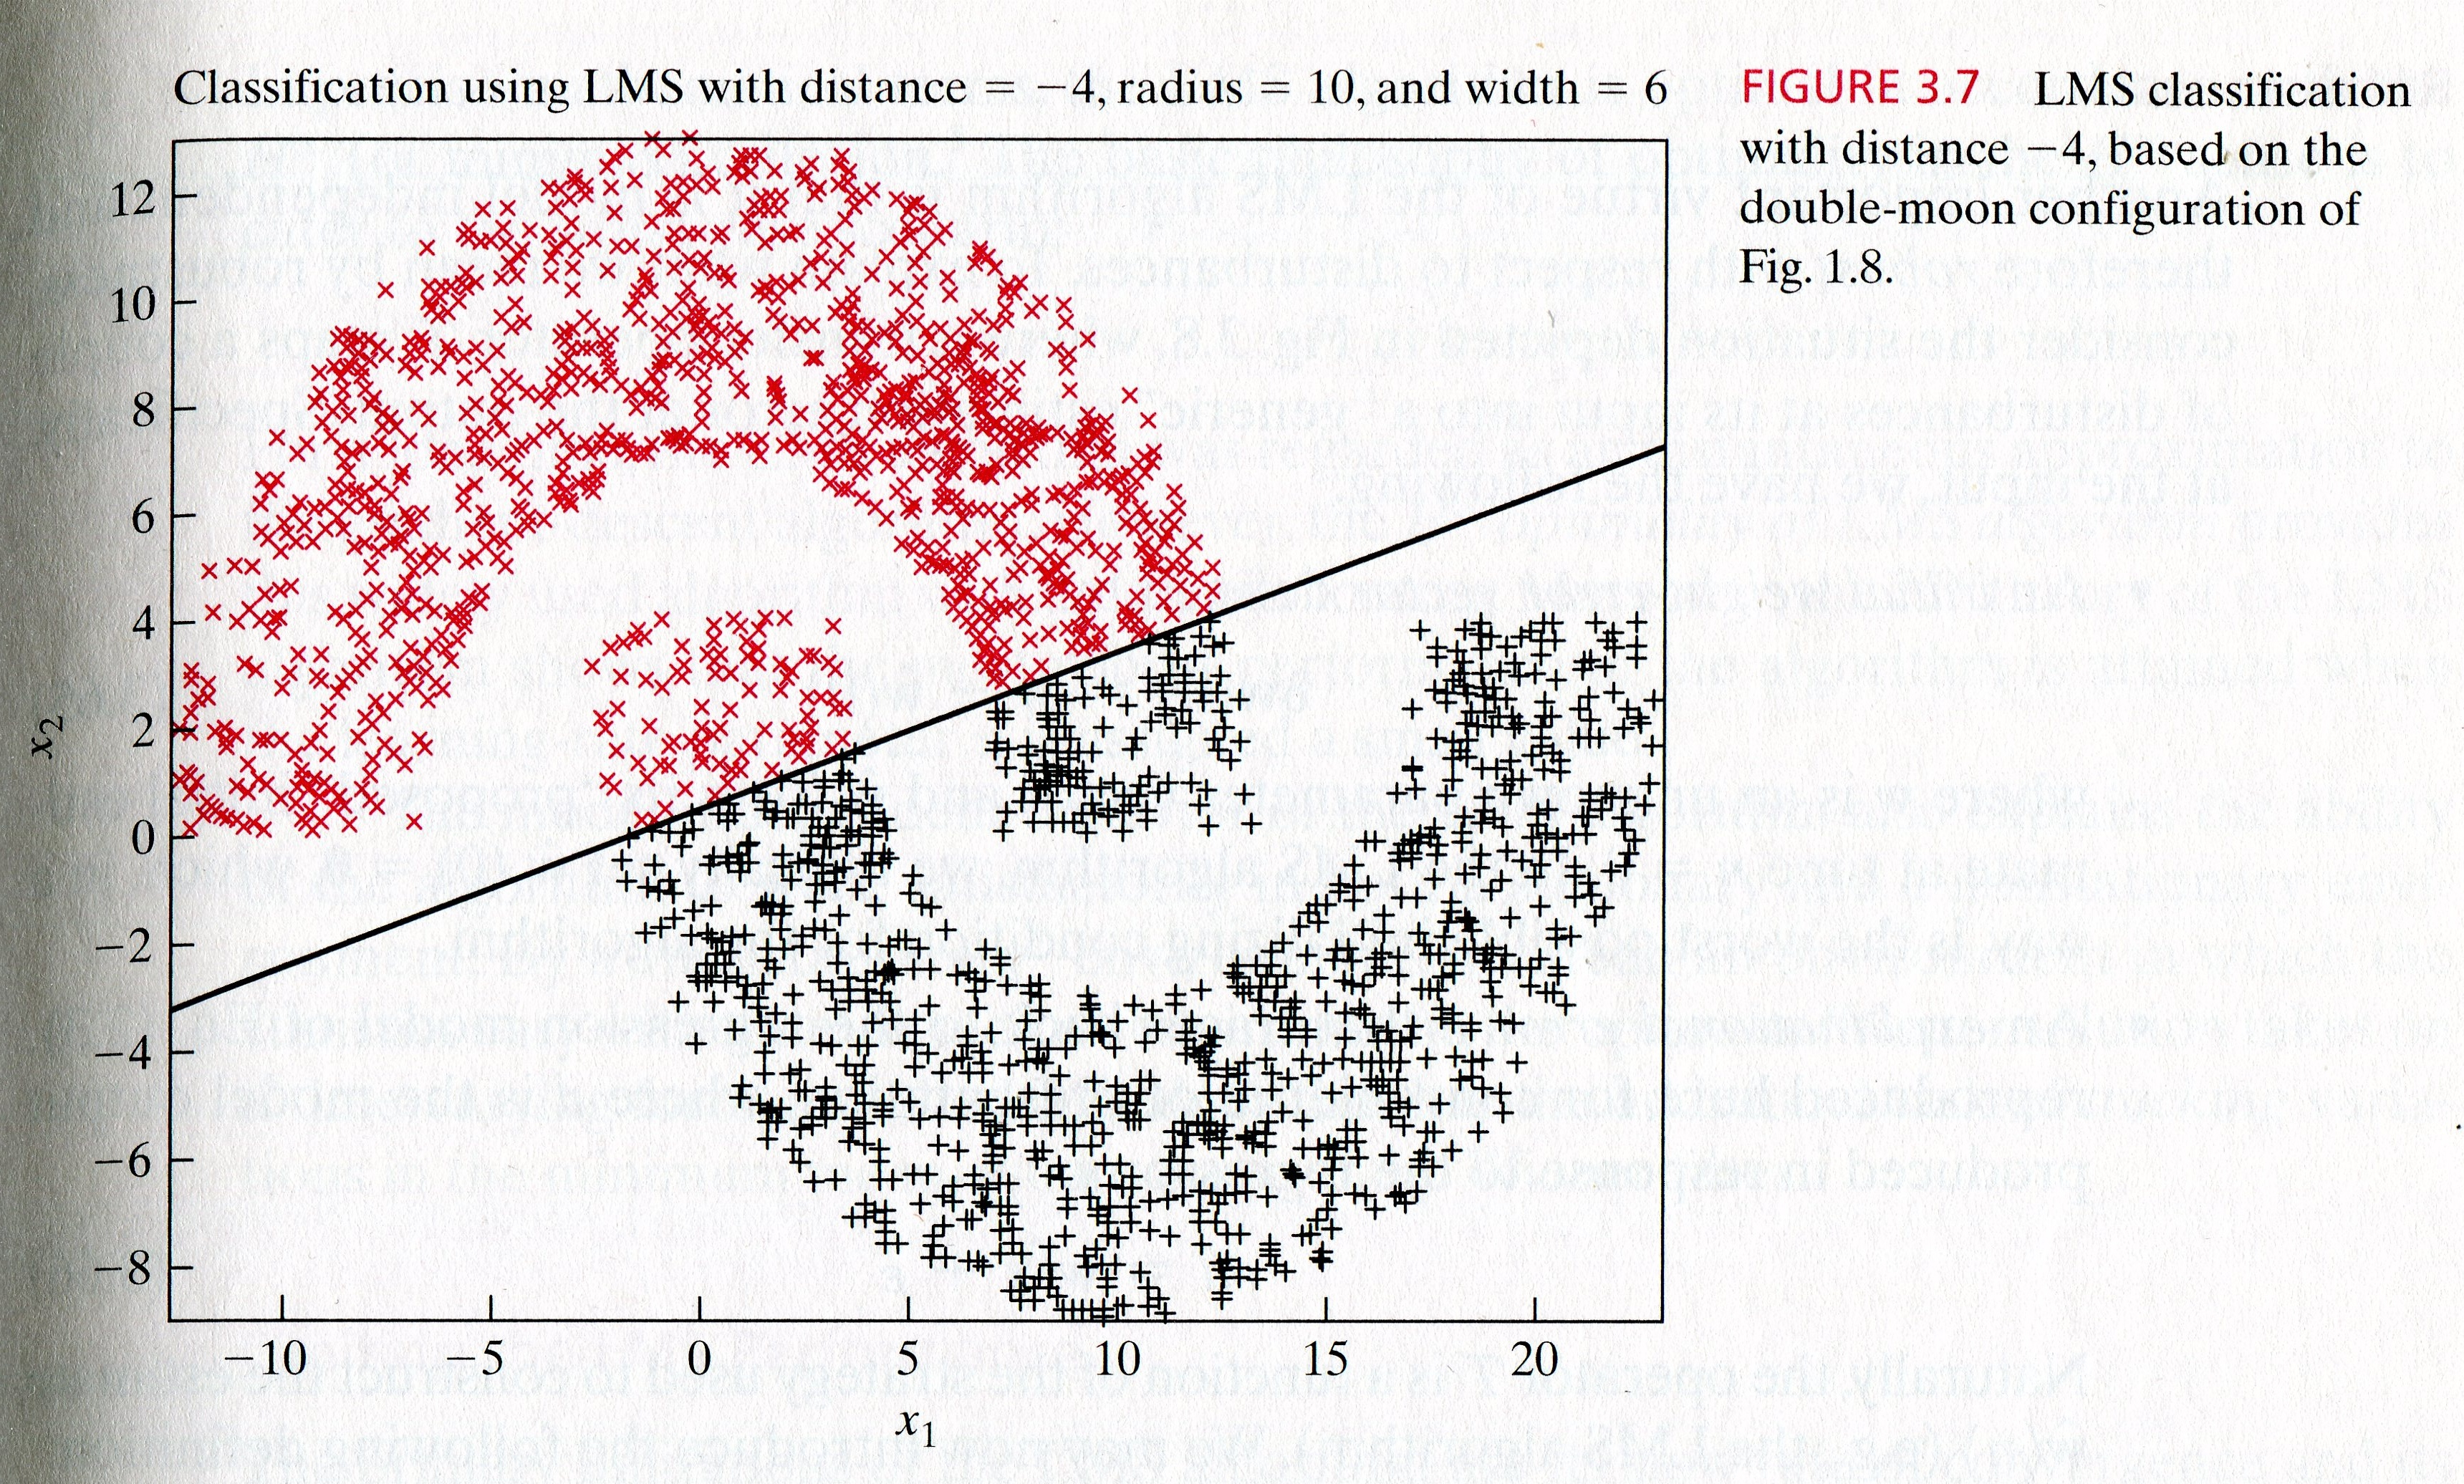
\includegraphics[width=0.7\linewidth]{ex07_04_lms.jpg}
      \\
      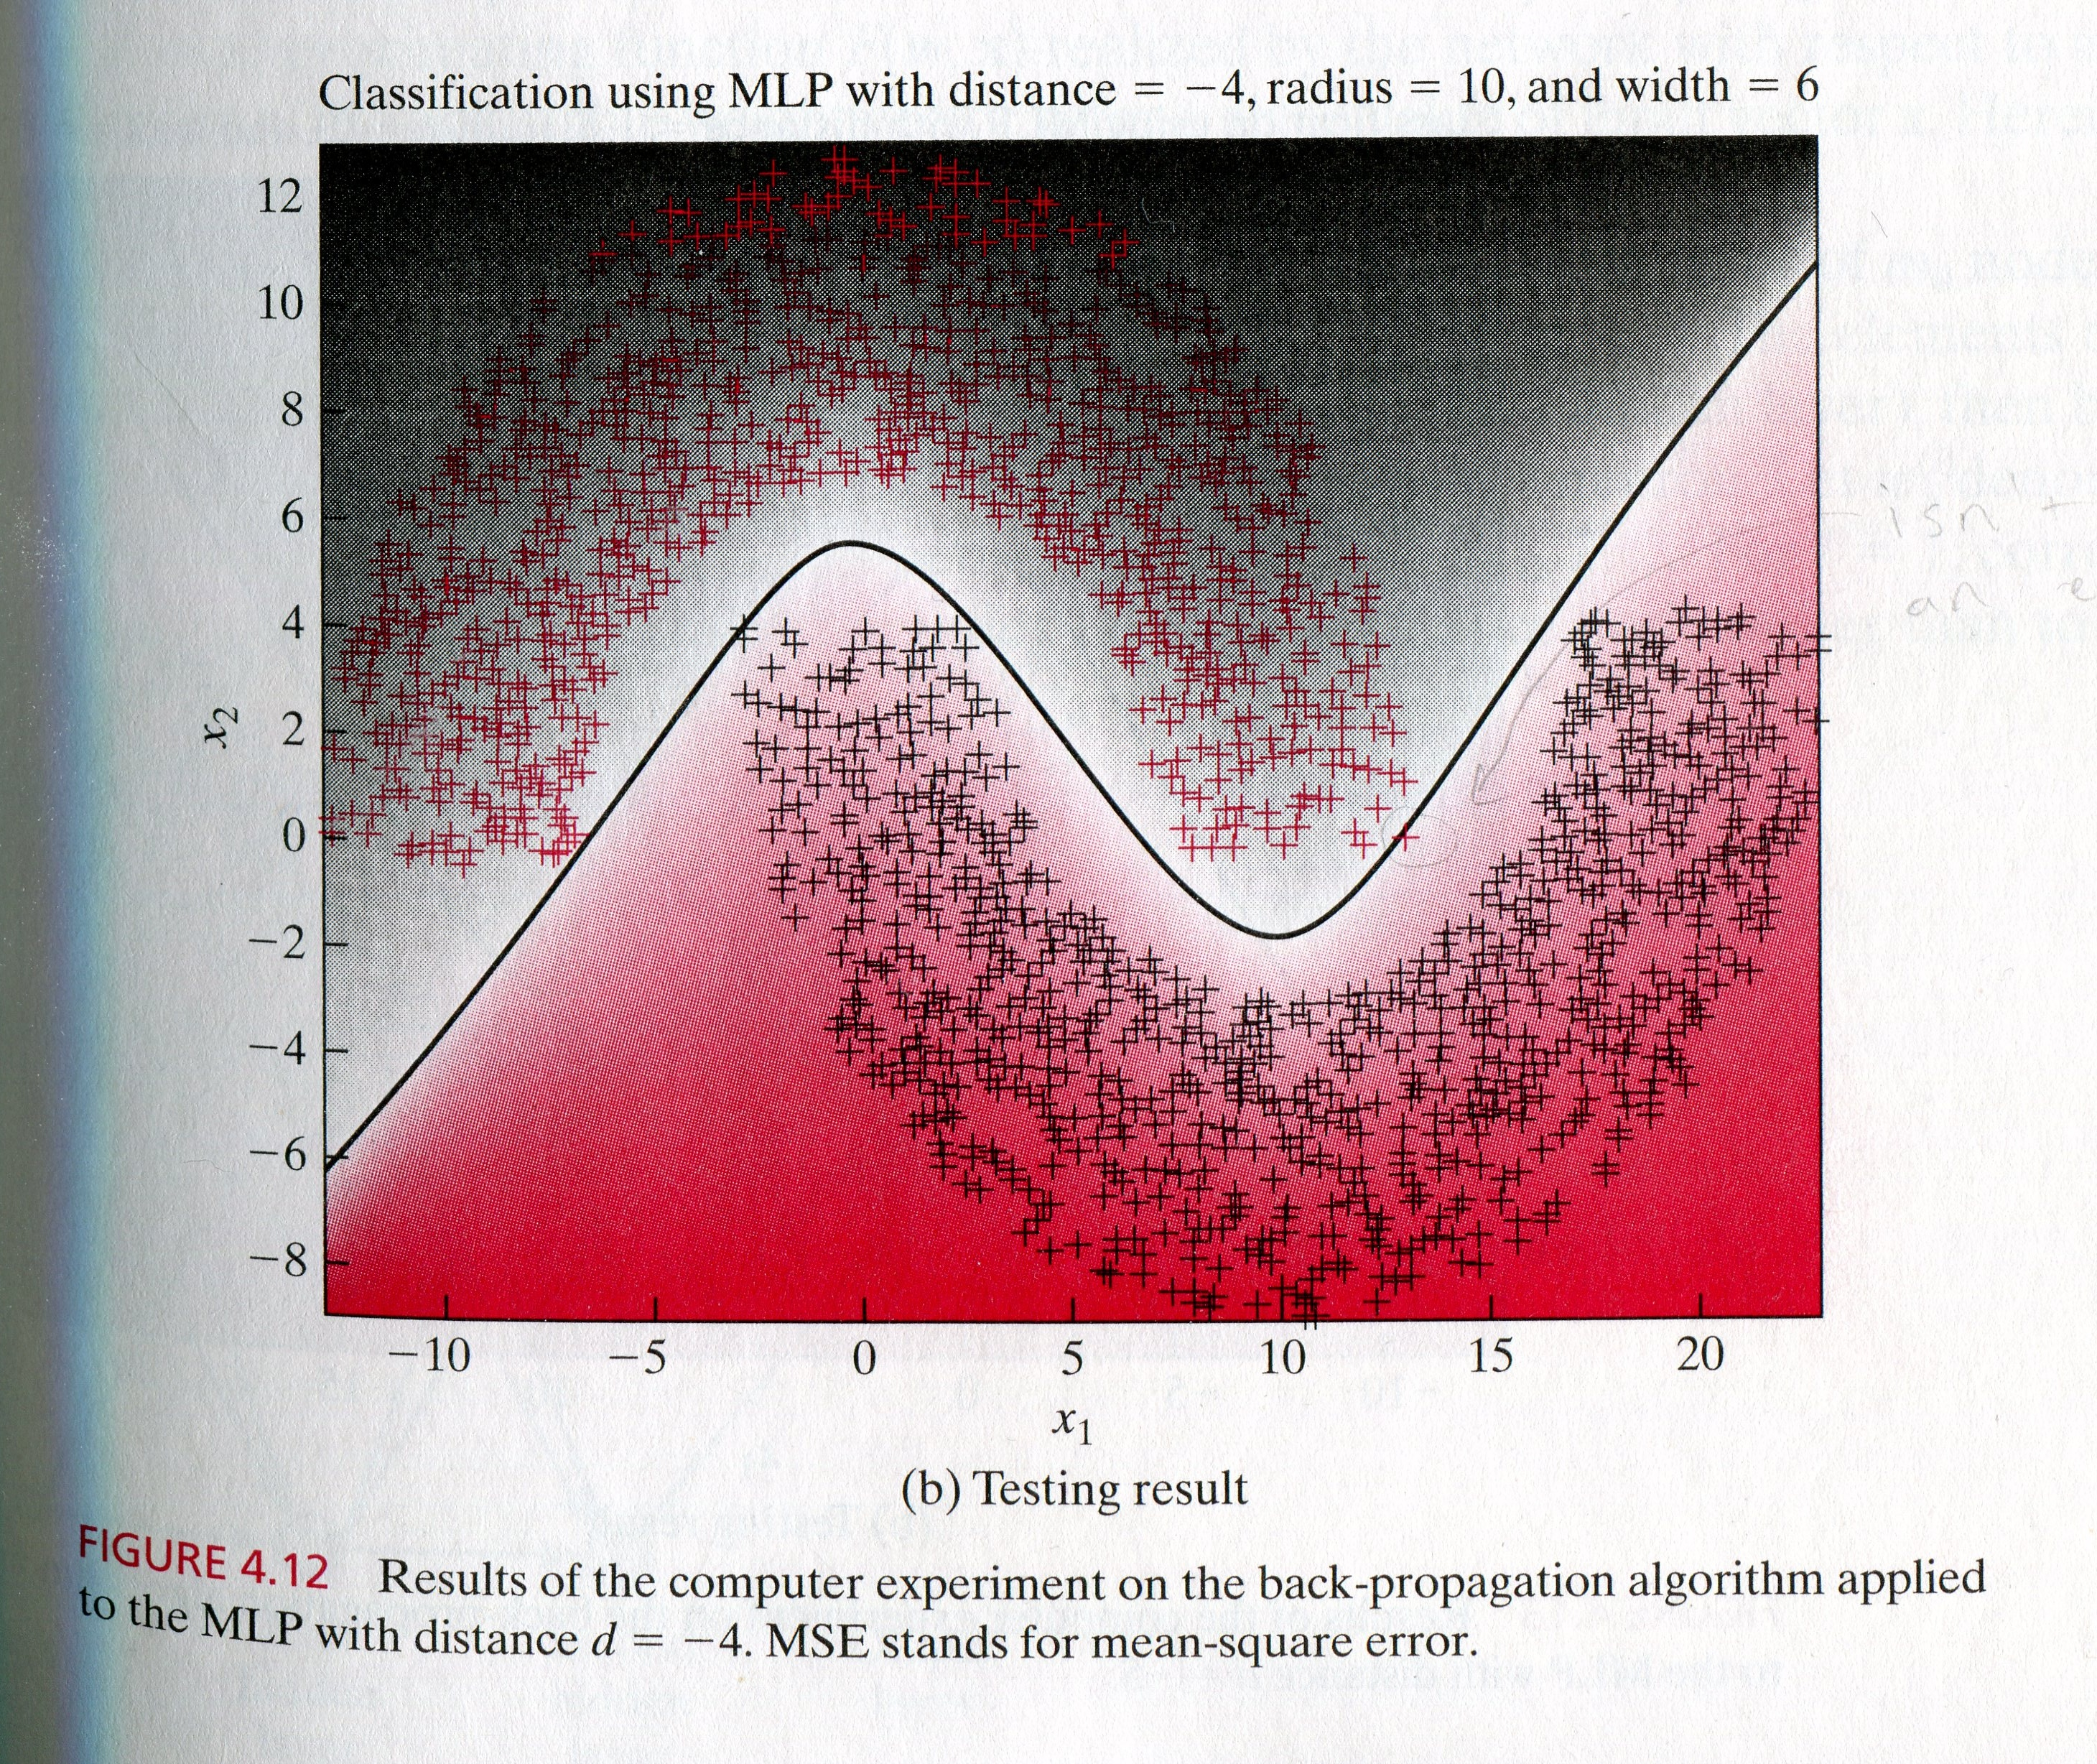
\includegraphics[width=0.7\linewidth]{ex07_04_mlp1.jpg}
      \\
      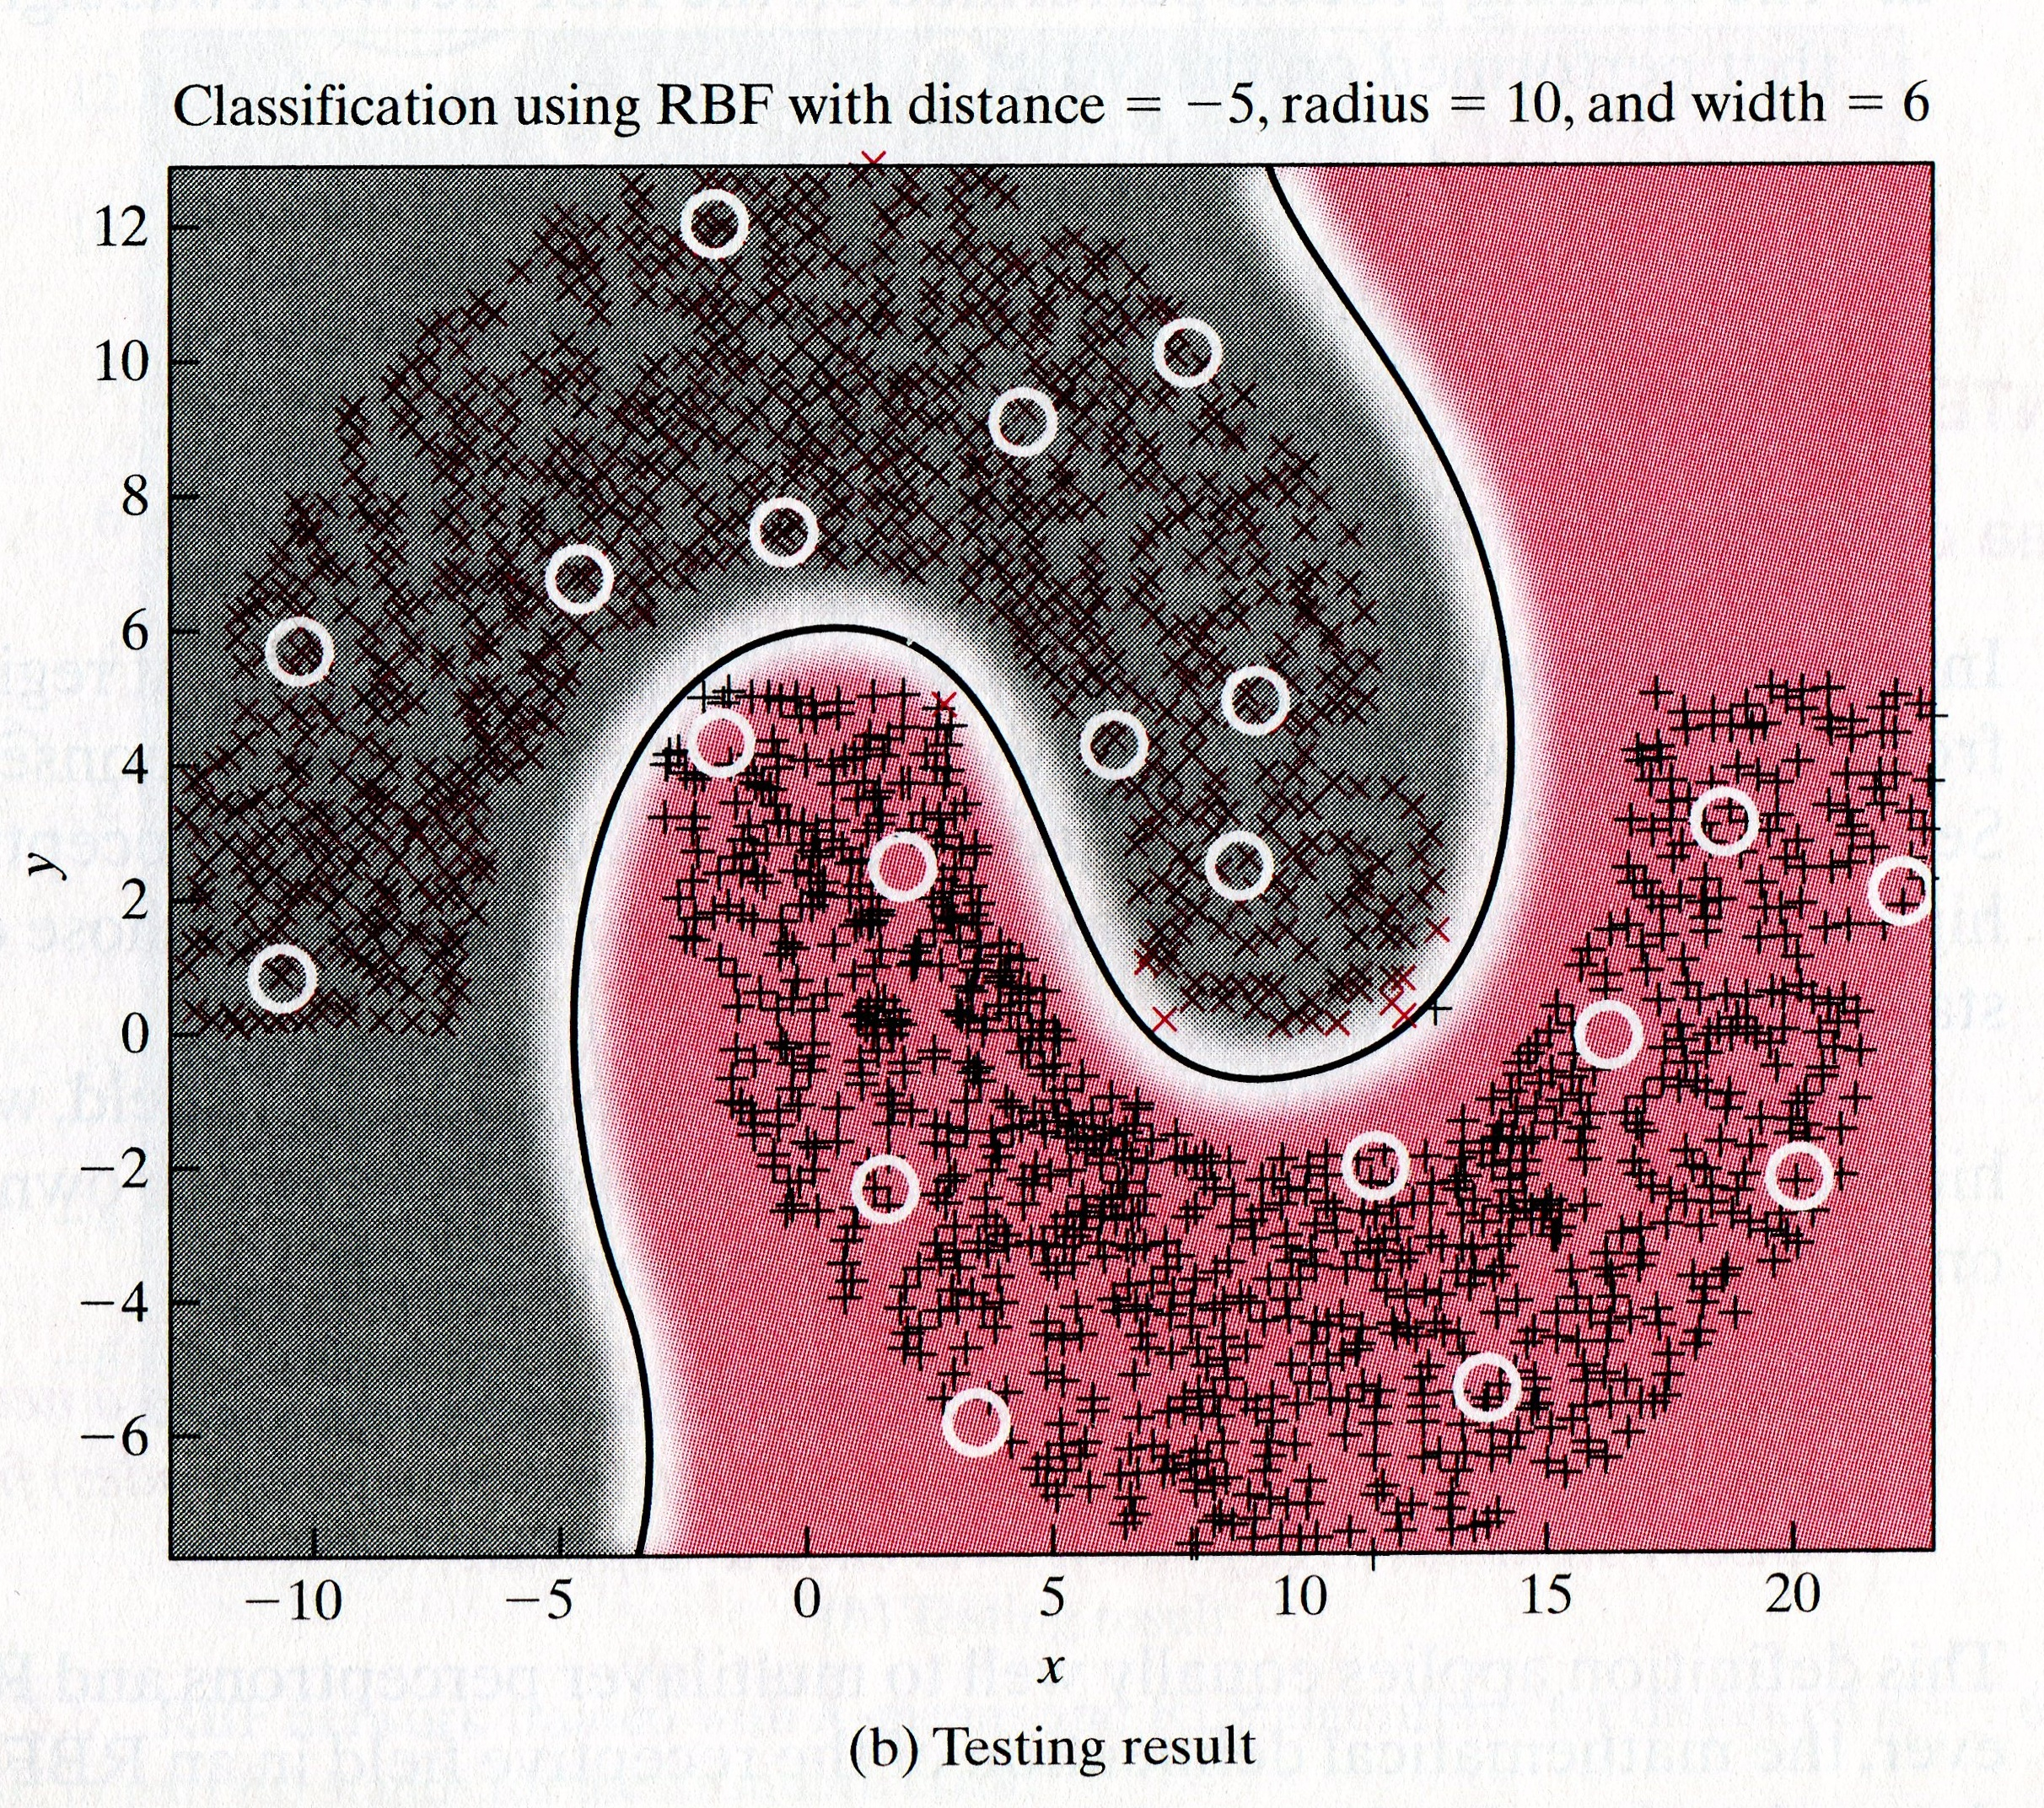
\includegraphics[width=0.7\linewidth]{ex07_04_rbf1.jpg}
    \end{center}
  \end{solution}
  
% \item Derive the learning rules for the stochastic gradient method for
%   training an RBF neural network.

%   \begin{solution}

%   \end{solution}
  
  
% \item Consider approximation of the nonlinear function $y = e^{-x} \sin(3x)$
%   on the interval $[0,4]$ using multilayer perceptron (MLP) and radial-basis
%   function (RBF) networks. Compare the generalization ability of these
%   networks.

%   \begin{solution}

%     See Ham \& Kostanic examples 3.2 and 3.4.
%   \end{solution}

  
  
\end{enumerate}
\end{document}             % End of document.

%%% Local Variables: 
%%% mode: latex
%%% TeX-master: "ex07_solutions"
%%% End: 
